\documentclass[11pt]{report}
\usepackage[utf8]{inputenc}
\usepackage[english]{babel}
\usepackage{graphicx}
\usepackage{fancyhdr}
\usepackage{color}
\usepackage{url}
\usepackage{fullpage}

\title{\huge{A Brief Tutorial on FreeRTOS} \\ and its port on the WSN430 hardware platform}
\author{Clément Burin des Roziers}

\begin{document}
   \maketitle

\abstract{This document presents a short introduction to the embedded real-time operating system FreeRTOS, how to port it on the WSN430 hardware platform, and gives some program examples easing the understanding of its features. This is by no mean a complete documentation on FreeRTOS. Such a document may be found on its official website : \url{http://www.freertos.org}}

   \tableofcontents

\chapter{Main Features of FreeRTOS}

FreeRTOS is a lightweight embeddable multi-task real-ime operating system. The produced kernel may require only a few kB of ROM and even less of RAM on the target microcontrolers, hence it is adapted for constrained embedded systems. The kernel source is developed in C language, thus reuse of existing C source code may be easily integrated. As a real-time OS, FreeRTOS focuses on multi-task scheduling and offers the following features:
\begin{itemize}
  \item cooperative, preemptive and hybrid scheduling;
  \item use of tasks and/or co-routines;
  \item multiple inter-tasks communication schemes (queues, semaphores, mutexes).
\end{itemize}

We will describe in deeper details these features now.

\section{Scheduling Modes}
The scheduling works with priorities. The running process will always be the one available with the highest priority. There are two scheduling schemes that may be implemented.
The first is preemptive, which means that a running process may be interrupted to let an other one be executed. The second is cooperative, which means that each process decides where in its execution it may be interrupted. When a process change is to be made, the scheduler chooses the one with the highest priority amongst those ready.

\section{Task Functionality}
A task is a process with its context. Therefore, several tasks can coexist in an application, but do not interfere with each other, they're independent. Since only one task can execute at a time, that is using the CPU, the scheduler swaps in and out the different tasks according to their priorities and the scheduling mode. A task states block diagram may be found in Fig.~\ref{task_diagram}.

\begin{figure}[ht]
\begin{center}
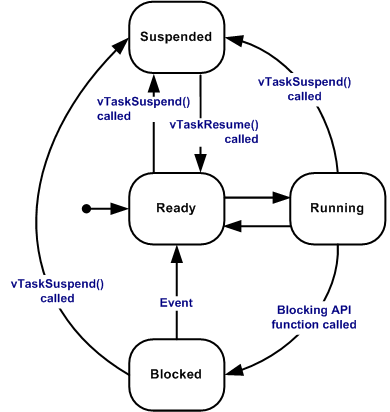
\includegraphics[scale=0.5]{figures/tskstate.png}
\end{center}
\caption{Task States Diagram}
\label{task_diagram}
\end{figure}

A task may be in different states. Here is a brief description of these states:
\begin{description}
	\item[Ready:] a task is ready when it just waits for the scheduler to give it access to the CPU, which means another task with higher or equal priority is running.
	\item[Running:] a task that is actually executing.
	\item[Blocked:] a task that waits for an event before continuing its execution. Events may be temporal (delay) or external (user interaction).
	\item[Suspended:] a task that has been removed from the scheduler. It will not be executed until it's put back to the Ready state.
\end{description}

The task priority is used by the scheduler to define which task to execute (put in the Running state). When several tasks are in the Ready state, it chooses the one with the highest priority. A task with a lower priority than another one will have to wait until this one enters the Blocked state to be executed.

A task is implemented as a function containing an infinite loop. This function should never returns.

There is a task that is systematically created in every application: the idle task. Defined with the lowest priority, it will be executed only when there is no other task in the Ready state. It is possible to define a function that will be called every time the idle task is entered (the idle task hook), which may be interesting for putting the device in a low power mode.

\section{Co-routine Functionality}
Co-routines are a different type of process that may be used for a real time application. The main differences with tasks are that co-routines use prioritized cooperative scheduling, which means they decide when another co-routine may be executed and they share a single stack which reduces the global RAM usage, but requires some special care. Their states diagram is found in Fig.~\ref{cr_diagram}.

\begin{figure}[ht]
\begin{center}
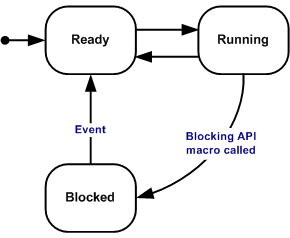
\includegraphics[scale=0.5]{figures/crstate.png}
\end{center}
\caption{Co-routine States Diagram}
\label{cr_diagram}
\end{figure}

A co-routine may be in the following states:
\begin{description}
	\item[Ready:] another co-routine or a task is Running.
	\item[Running:] the co-routine is executing.
	\item[Blocked:] the co-routine is waiting for an event to be Ready again.
\end{description}

The co-routines of an application are prioritized, that is when the scheduler have to choose a co-routine to execute it will take the one in the Ready state with the highest priority. When tasks and co-routines are use simultaneously in an application, any task will always take priority over co-routines. 

\section{Intertask Communication}
\subsection{Queues}

Queues are the generic form of intertask communications. They are FIFO buffers that may be accessed (read from and written to) by tasks. The items placed in the queues are of fixed size, defined with the maximum number of elements when the queue is created.

Reads and writes to the queue are done by copy, therefore the larger the elements are, the more memory will be required by the queue. It is possible to place pointers in the queue, care must then be taken not to modify the data before it is read.

Tasks can block on queues, waiting for an item to be inserted, or space to be made. It is a way to synchronize different tasks between them, or with interrupts.

\subsection{Semaphores}
Semaphores are directly derived from queues, and contains only one element. The queue can be full or empty and what's contained in the queue doesn't matter.

A task can 'take' a semaphore, that is emptying the queue. If the queue wasn't full, it will block. An interrupt can 'give' the semaphore, that is filling the queue, hence allowing the task to continue.

Semaphores are therefore mainly designed to offer synchronization between tasks and interrupts.

\subsection{Mutexes}

Mutexes (for MUTual EXclusion) are a form of binary semaphores used to prevent several Tasks to access the same resource at the same time. A mutex is created for a shared resource and it's associated queue is full. When a task wants to access the resource, it 'takes' the mutex. When the task is done with the resource, it gives the mutex back, so another task can use it. If a task tries to take a mutex that is already taken, it will block until it's given back.

\chapter{Porting FreeRTOS on the WSN430 hardware platform}
\section{Option 1: Do It Yourself}
If you want to be sure to use the latest available version of FreeRTOS, you can adapt the kernel source files for the msp430f1611 manually as follows.

Download the latest archive from \url{www.freertos.org} and extract it. The FreeRTOS source files organization is as follows: there are two important folders. One is 'Source', it contains the four common files to every architecture with their headers, and the 'portable' folder containing processor specific ports. The other, Demo, contains examples programs for a lot of hardware platforms.

There exists a port of FreeRTOS for the msp430f449 microcontroller on some hardware platform. Thus a few modifications need to be done in order to port it for the WSN430 platform. The port specific source files located in  the 'Source/portable/GCC/MSP430F449' directory are completely compatible with the msp430f1611. Since it is easier to use it directly without renaming it, that's what we'll do. The code in this folders contain processor specific functions (such as configuration of the timer responsible for the scheduler tick interrupt.

We are now going to port the demo application to the WSN430 platform. Copy now the folder 'Demo/msp430\_GCC' to 'Demo/WSN430\_GCC'. There are a few files in it: main.c is the main source code that contains the main function. That's where the tasks will be created and the scheduler started. The file 'FreeRTOSConfig.h' contains a lot of configurations fields allowing the user to specify the characteristics of the kernel. Must be specified the speed of the main clock, the desired tick rate, the available memory on the target and the maximum number of priorities for example. Finally the file 'makefile' contains the compiling directives.

The two directories 'ParTest' and 'serial' contain code for the demo application allowing to control the LEDs and a serial communication respectively. In our first tiny program, we won't need them, they can be deleted. (For information, the target board of the initial port didn't have LEDs but some LCD segments. It is more time consuming to adapt all the existing functions that to rewrite them)

\begin{description}
  \item[FreeRTOSConfig.h] the included header (\#include <msp430x44x.h>) at the top of the file is not for the same msp430. For simplicity, it may be replaced by \#include <io.h>. Next the CPU clock frequency contained in the field configCPU\_CLOCK\_HZ should be updated to 8000000 (8MHz). The tick rate is set to 1000Hz, which is fine, and the heap size may be updated for the new msp430, that is 9800 bytes (out of 10kB RAM).

  \item[makefile] Here we need to update the mmcu used by the compiler by replacing '-mmcu= msp430x449' with '-mmcu= msp430x1611' in the CFLAGS line. We don't have to do the same for the PORT\_PATH line by replacing MSP430F449 since we saw above that the included source files works for both architectures. Finally in the SRC list, we'll need just the minimal, hence we can remove the lines corresponding to ParTest, serial, flash, integer, comtest and PollQ.

  \item[main.c] In the main file, the easiest is to erase everything and start from scratch. We'll go from top to bottom. The required includes are :
\begin{verbatim}
/* Scheduler includes. */
#include "FreeRTOS.h"
#include "task.h"
\end{verbatim}

Then we need some 'define' for simple LEDs handling:
\begin{verbatim}
/* LEDs config */
#define mainLED_TASK_PRIORITY (tskIDLE_PRIORITY + 1)
#define LED_OUT   P5OUT
#define BIT_BLUE   (1 << 6)
#define BIT_GREEN  (1 << 5)
#define BIT_RED    (1 << 4)
\end{verbatim}

Then the file's prototypes:
\begin{verbatim}
/* 
 * The LEDs flashing tasks
 */ 
static void vTaskLED0( void *pvParameters );
static void vTaskLED1( void *pvParameters );
static void vTaskLED2( void *pvParameters );
/*
 * Perform Hardware initialization.
 */
static void prvSetupHardware( void );

\end{verbatim}
And the main function:
\begin{verbatim}
int main( void )
{
  /* Setup the hardware ready for the demo. */
  prvSetupHardware();
  
  /* Start the LEDs tasks  */
  xTaskCreate( vTaskLED0, "LED0", configMINIMAL_STACK_SIZE, \
     NULL, mainLED_TASK_PRIORITY, NULL );
  xTaskCreate( vTaskLED1, "LED1", configMINIMAL_STACK_SIZE, \
     NULL, mainLED_TASK_PRIORITY, NULL );
  xTaskCreate( vTaskLED2, "LED2", configMINIMAL_STACK_SIZE, \
     NULL, mainLED_TASK_PRIORITY, NULL );

  /* Start the scheduler. */
  vTaskStartScheduler();

  /* As the scheduler has been started the demo application
  tasks will be executing and we should never get here! */
  return 0;
}
\end{verbatim}

We have now to develop the task functions:
\begin{verbatim}
/* First LED flash task */
static void vTaskLED0( void *pvParameters )
{
  while (1)
  {
    /* Toggle blue LED and wait 500 ticks */
    LED_OUT ^= BIT_BLUE;
    vTaskDelay(500);
  }
}

/* Second LED flash task */
static void vTaskLED1( void *pvParameters )
{
  while (1)
  {
    /* Toggle green LED and wait 1000 ticks */
    LED_OUT ^= BIT_GREEN;
    vTaskDelay(1000);
  }
}

/* Third LED flash task */
static void vTaskLED2( void *pvParameters )
{
  while (1)
  {
    /* Toggle red LED and wait 2000 ticks */
    LED_OUT ^= BIT_RED;
    vTaskDelay(2000);
  }
}
\end{verbatim}

And finally the hardware setup function:
\begin{verbatim}
static void prvSetupHardware( void )
{
  /* Stop the watchdog timer. */
  WDTCTL = WDTPW + WDTHOLD;

  /* Setup MCLK 8MHz and SMCLK 1MHz */
  DCOCTL  = 0;
  BCSCTL1 = 0;
  BCSCTL2 = SELM_2 | (SELS | DIVS_3) ;

  /* Wait for cristal to stabilize */
  int i;
  do {
    /* Clear OSCFault flag  */
  	IFG1 &= ~OFIFG;
    /* Time for flag to set */
  	for (i = 0xff; i > 0; i--) nop();
  } while ((IFG1 & OFIFG) != 0);

  /* Configure IO for LED use */
  P5SEL  &= ~(BIT_BLUE | BIT_GREEN | BIT_RED);
  P5OUT  &= ~(BIT_BLUE | BIT_GREEN | BIT_RED);
  P5DIR  |=  (BIT_BLUE | BIT_GREEN | BIT_RED);
}
\end{verbatim}

\end{description}

That's it! Now you should be able to compile and load the program to the target, assuming required software (mspgcc) and hardware (JTAG FET) are installed and working.
The three LEDs should be blinking at different rates!

\section{Option 2: Use It Ported (recommended)}
The other and simpler way is to directly use the ported source files found in the \verb$kernel$ directory. In it are two sub-folders, \verb$Source$ that contains the FreeRTOS kernel source, and \verb$Demo$ that contains one program example directly working on the WSN430. (This demo corresponds to the one described above)

\section{Programming Remarks and Advices}
When using FreeRTOS as the OS for an application on the WSN430 platform, a few points need special attention.

\subsection{FreeRTOS Tick}
The real time aspect of the OS is based on counting ticks. An MMCU internal timer is used to generate an interrupt periodically allowing the OS to count time, to preempt tasks and offer a delay mechanism. The default configuration of the OS is to use the timerA of the msp430, configured with the ACLK source clock (assumed to be 32768Hz). In the \verb$FreeRTOSConfig.h$ file required in every application, the desired tick rate is specified. If a tick rate of 1kHz is wanted, the timerA CCR register will be set to 32768/1000 = 32, therefore the real tick rate will be 1024Hz.

To sum up, when using FreeRTOS:
\begin{itemize}
	\item do not use the timerA on your own, it's already used by the kernel;
	\item be careful if your application require accurate time measurement, the division rounding may result in erroneous values;
	\item set ACLK to be 32768Hz. On the WSN430 platform, ACLK should be derived from XT1 with a divider of 1.
\end{itemize}

\subsection{Shared Buses}
On the WSN430 platform, several peripherals communicate with the msp430 using shared buses. There are two communication buses on the msp430f1611: USART0 and USART1. On the USART0 are the TSL2550 light sensor using I$^2$C and a serial link with a PC (or equivalent) using UART. On the USART1 are the CC1100 radio chip using SPI, the M25P80 flash memory using SPI, the DS1722 temperature sensor using SPI and a serial link with a PC (or equivalent) using UART.

Each of these USARTs can be configured for on type of link at a time (UART/SPI/I$^2$C), thus if you want to switch between several peripherals on the same port, you have to reconfigure it before using it (calling the \verb$xxx_init()$ function of the driver might do the trick). On the USART1, three peripherals can be accessed using SPI. With this type of bus, the different devices share the same communication link, but are enabled/disabled using separate lines. When communicating with a device, the other devices on the same SPI bus must be disabled, that is: only one device should be enabled at a time. To do this, the \verb$spi1.h$ driver disable the other two SPI peripherals when enabling one.

In a multitask environment, if two tasks want to access two different devices on the same SPI bus, care must be taken in order to not interrupt a given transfer, and a mutex (mutual exclusion semaphore) should be used for this. FreeRTOS offers a simple way of using a mutual exclusion semaphore, therefore it is recommended to use it.

The same way, mutexes should be used to prevent different tasks interfering with each other accessing the different msp430 USART ports.


\chapter{Program examples}

In this chapter, we're going to build an entire application from \textit{almost} scratch, using FreeRTOS as the OS on the nodes. Here are the main elements of the application:
\begin{description}
	\item[sensor node:] a remote node may sample light and temperature with its integrated sensors, as well as light its three LEDs;
	\item [sink node:] another node sends commands to and receives data from the remote sensor node;
	\item [PC:] a computer with a user application sends the commands and retrieve the data from the sink node via a serial link.
\end{description}
The total application schema is found in Fig.~\ref{fig:archi}.

\begin{figure}[ht]
	\begin{center}
	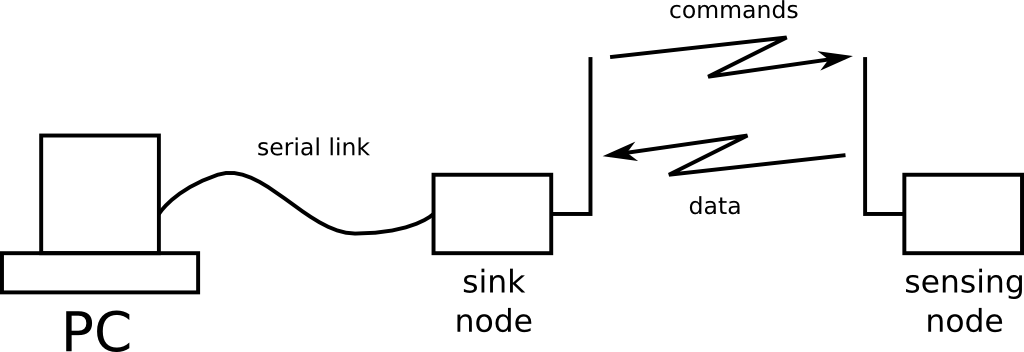
\includegraphics[width=0.8\textwidth]{figures/archi.png}
	\end{center}
	\caption{Application overview}
	\label{fig:archi}
\end{figure}

The different communications that take place over the air are:
\begin{itemize}
	\item LED commands to light on/off the different sensor node LEDs;
	\item sensor commands to chose the sensors to sample, the sample rate, and the number of samples per packet to be sent back to the sink node;
	\item data from sampled sensors.
\end{itemize}

We'll go through all the required steps to build the firmware of the sensor and sink nodes in the next sections.

\section{Sensor Node Firmware}

\subsection{Tasks}
The different functionalities of the sensor node are the following:
\begin{description}
	\item[sensing:] sample periodically the chosen sensors, gather the samples in packets ready to be sent. Adjust the sampling parameters according to received commands;
	\item[lighting:] switch the LEDs on/off according to the received commands;
	\item[communicating:] receive the different commands, decode them and execute them. Send the sampled data to the sink node.
\end{description}

Hence we divide the overall application in three different tasks, corresponding to the three main functions of the node. The tasks' priorities depend on their timing requirements:

The \textbf{blinker} task, responsible for switching on/off the LEDs has the least requiring timing, therefore we'll attribute it the smallest priority.

The \textbf{sensor} task, responsible for sampling the sensors, must execute periodically and not get delayed too much. It's priority will be higher than the blinker's one.

the \textbf{mac} task, implementing a simple MAC layer allowing the node to communicate must be very reactive to incoming and outgoing communications, therefore it will have the highest priority.

The corresponding task priorities are shown in Fig.~\ref{fig:prio}

\begin{figure}[ht]
	\begin{center}
	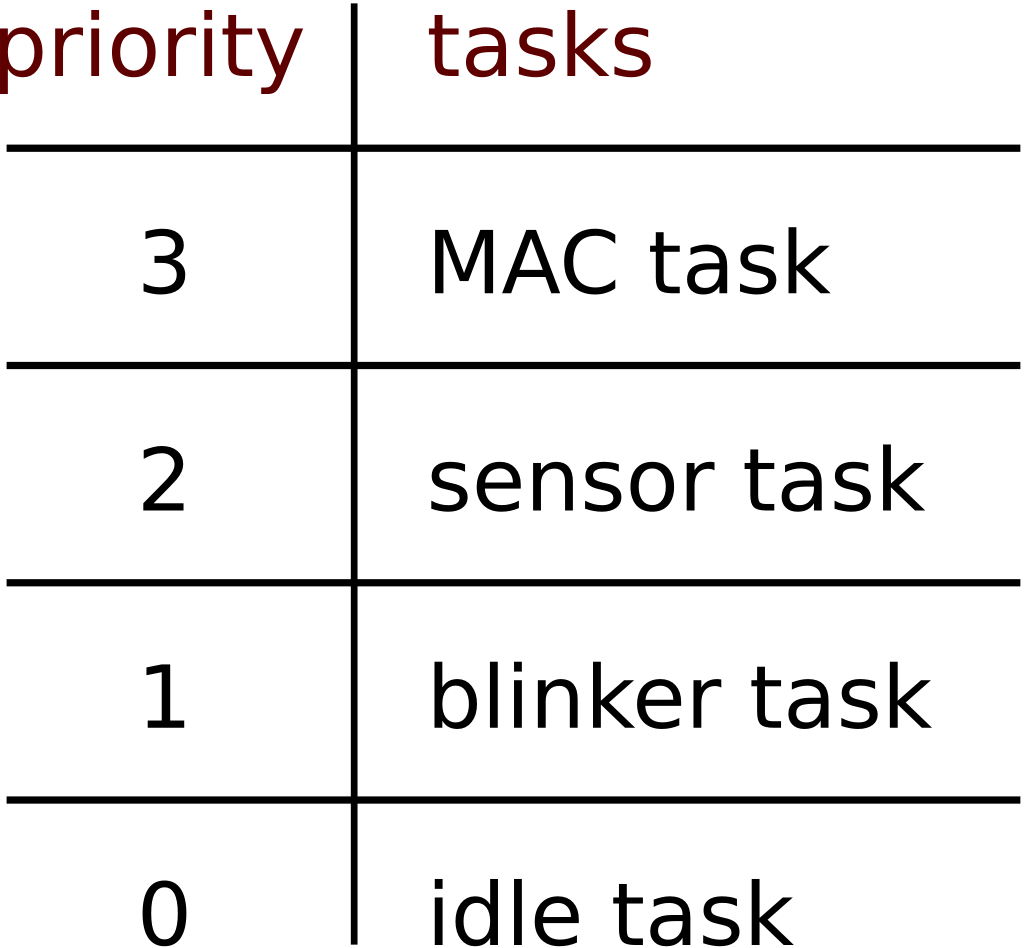
\includegraphics[scale=1]{figures/prio.png}
	\end{center}
	\caption{Task Priorities}
	\label{fig:prio}
\end{figure}

\subsection{Intertask Communication}
Now we've defined roughly what the tasks have to do, we need to consider how the task communicate with each other. As we've seen above, the mac task will receive commands sent to the blinker and the sensor tasks. As it needs to transfer the command to the desired task, we have to add a way to pass messages between the mac task and the other tasks. That's what is done with queues.
Thus for passing received commands to the corresponding tasks, we'll create two queues, one for mac->blinker communications and one for mac->sensor communications. On the other way around, the sensor task gathers samples in packets, and sends them, hence there must be a queue for passing packets from the sensor task to the mac task.

To sum up, three queues are needed by this application:
\begin{itemize}
	\item mac-\textgreater blinker for passing LED relative received commands;
	\item mac-\textgreater sensor for passing sampling configuration received commands;
	\item sensor-\textgreater mac for passing sampled data to send to the sink node.
\end{itemize}

In Fig.~\ref{fig:queues} is found a schema representing the tasks and queues.

\begin{figure}[ht]
	\begin{center}
	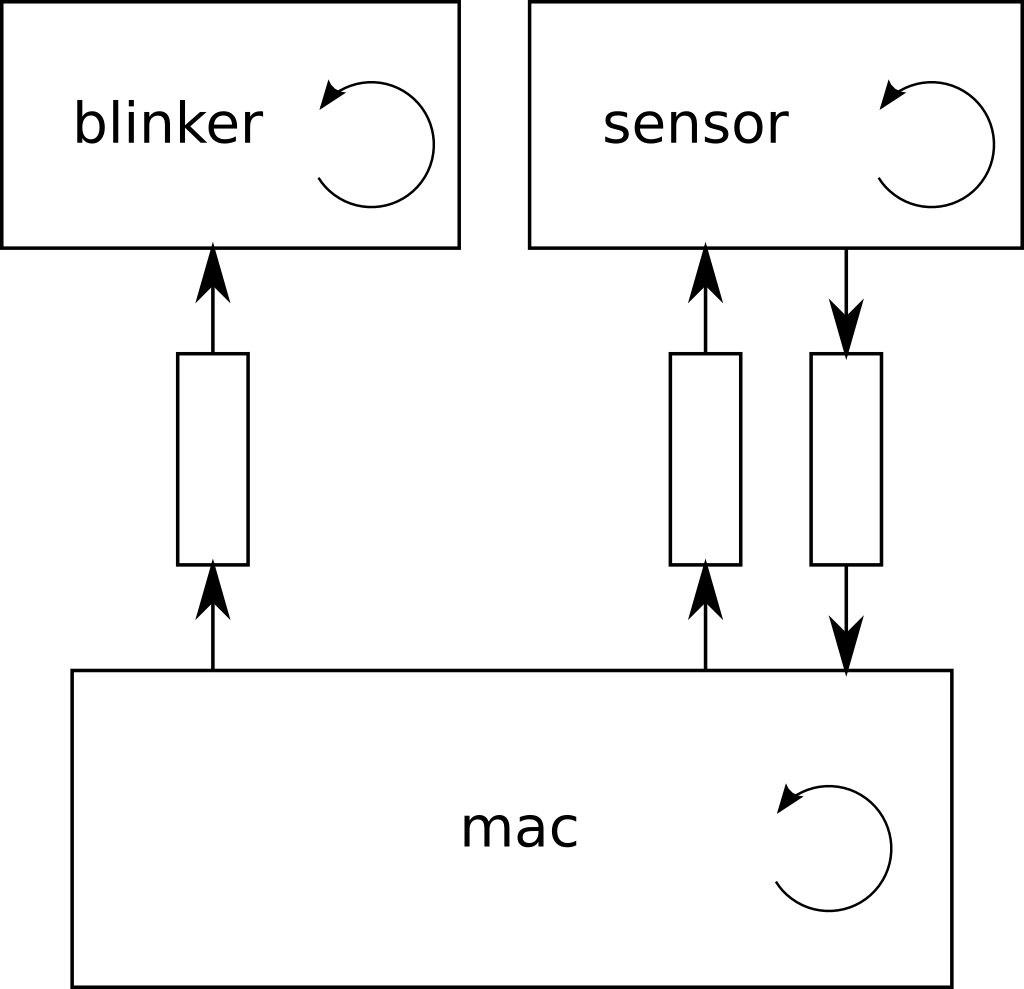
\includegraphics[scale=.8]{figures/queues.png}
	\end{center}
	\caption{Tasks and Queues}
	\label{fig:queues}
\end{figure}

\subsection{Source Files Organization}

The sensor node firmware is found in the \verb$node_example$ folder, and is organized as follows. In the project root folder are the files:
\begin{itemize}
	\item FreeRTOSConfig.h: contains OS specific constant parameters.
	\item queue\_types.h: contains the item types for the different queues.
	\item main.c : source code containing the initialization procedure. It creates the required queues, tasks, and starts the scheduler.
	\item makefile: contains the compilation instructions.
\end{itemize}

The blinker sub-folder contains all the files about the blinker task:
\begin{itemize}
	\item blinker.h: header file containing the task initialization function prototype, called from main.c.
	\item blinker.c: the source file for the blinker task.
\end{itemize}

The sensor sub-folder contains all the files about the sensor task:
\begin{itemize}
	\item sensor.h: header file containing the task initialization function prototype, called from main.c.
	\item sensor.c: the source file for the sensor task.
\end{itemize}


The mac sub-folder contains all the files about the mac task:
\begin{itemize}
	\item mac.h: header file containing the task initialization function prototype, called from main.c.
	\item mac.c: the source file for the mac task.
\end{itemize}

\subsection{The blinker Task}
This is a very simple task, since it must just wait until a command is received, and execute it. The initialization function prototype of the header file is:
\begin{verbatim}
void vCreateBlinkerTask(xQueueHandle xQueue, uint16_t usPriority);
\end{verbatim}
Where xQueue is the queue handler by which the commands are received, and usPriority is the priority that should have the blinker task.

The blinker module contains three functions. The first is \verb$vCreateBlinkerTask$ as described above that initiates the task. The second is \verb$vBlinkerTask$, it's the task itself, that should contains an infinite loop and never returns. The third is \verb$vParseAndExecute$, which is called every time a command is received.

Lets see these functions in detail.

\begin{verbatim}
void vCreateBlinkerTask(xQueueHandle xQueue, uint16_t usPriority)
{
    /* Store the command queue handle */
    xCmdQueue = xQueue;
    
    /* Create the task */
    xTaskCreate( vBlinkerTask, "blinker", configMINIMAL_STACK_SIZE, NULL, usPriority, NULL );
}
\end{verbatim}
This function just stores the queue handle in a variable, and creates the task with the argument-given priority.

\begin{verbatim}
static void vBlinkerTask(void* pvParameters)
{
    rxdata_t rx_data;
    
    /* Configure and Initialize the LEDs */
    LEDS_INIT();
    LEDS_ON();
    
    for (;;)
    {
        /* Wait until a command is received */
        if (xQueueReceive(xCmdQueue, (void*) &rx_data, portMAX_DELAY))
        {
            vParseAndExecute(rx_data.cmd);
        }
    }
\end{verbatim}

This task function initiates the LED driver, and repeatedly waits for a command to be inserted in the queue and handles it with the next function:

\begin{verbatim}
void vParseAndExecute(uint8_t cmd)
{
    switch (cmd & CMD_MASK)
    {
        case CMD_LED_ON:
            switch (cmd & LED_MASK)
            {
                case LED_RED:
                    LED_RED_ON();
                    break;
                case LED_GREEN:
                    LED_GREEN_ON();
                    break;
                case LED_BLUE:
                    LED_BLUE_ON();
                    break;
                case LED_ALL:
                    LEDS_ON();
                    break;
            }
            break;

        case CMD_LED_OFF:
            switch (cmd & LED_MASK)
            {
                case LED_RED:
                    LED_RED_OFF();
                    break;
                case LED_GREEN:
                    LED_GREEN_OFF();
                    break;
                case LED_BLUE:
                    LED_BLUE_OFF();
                    break;
                case LED_ALL:
                    LEDS_OFF();
                    break;
            }
            break;
        case CMD_LED_TOGGLE:
            switch (cmd & LED_MASK)
            {
                case LED_RED:
                    LED_RED_TOGGLE();
                    break;
                case LED_GREEN:
                    LED_GREEN_TOGGLE();
                    break;
                case LED_BLUE:
                    LED_BLUE_TOGGLE();
                    break;
                case LED_ALL:
                    LED_RED_TOGGLE();
                    LED_GREEN_TOGGLE();
                    LED_BLUE_TOGGLE();
                    break;
            }
            break;
        case CMD_LED_BLINK:
            /* Not Implemented */
            break;
    }
\end{verbatim}
This function takes the received command and parses it. According to its content, the desired LED is switched on/off or toggled.

\subsection{The sensor Task}
The main activity of this task is to sample and store periodically the light and temperature sensors according to the required configuration. The other thing this task has to do is to check if a command has been received to change the sampling characteristics.

The initialization function prototype found in the header file is:

\verb$void vCreateSensorTask(xQueueHandle xSensorCmdQueue, xQueueHandle xMacDataQueue, uint16_t usPriority);$

Where xSensorCmdQueue is a handle of the queue for receiving commands, xMacDataQueue is a handle to the queue for sending data and usPriority is the priority the task should run at.

The sensor modules contains five functions,\verb$vCreateSensorTask$ as seen above is used to add the task to the scheduler, \verb$vSensorTask$ is the task function that contains the task loop, \verb$vSampleSensors$ is the function that reads the values from the sensors and store them at the right place, \verb$vSendData$ is the function that place the gathered data in the queue, in order to send it to the mac task, and finally \verb$vParseAndExecute$ is used to analyze a received command and change the task settings accordingly.

Let's step through these functions:
\begin{verbatim}
void vCreateSensorTask(xQueueHandle xSensorCmdQueue, xQueueHandle xMacDataQueue, uint16_t usPriority)
{
    /* Store the command and data queue handles */
    xCmdQueue = xSensorCmdQueue;
    xDataQueue = xMacDataQueue;
    
    /* Create the task */
    xTaskCreate( vSensorTask, "sensor", configMINIMAL_STACK_SIZE, NULL, usPriority, NULL );
}
\end{verbatim}

The initialization function stores the queue handles, and add the task in the scheduler.

\begin{verbatim}
static void vSensorTask(void* pvParameters)
{
    portTickType xLastSampleTime;
    rxdata_t rx_data;
    
    /* Setup the ds1722 temperature sensor */
    ds1722_init();
    ds1722_set_res(12);
    ds1722_sample_cont();

    /* Setup the TSL2550 light sensor */
    tsl2550_init();
    tsl2550_powerup();
    
    blockOnCmd = 1;
    activeSensors = SENSOR_NONE;
    packet.sequence = 0;
    filling_index = 0;
    
    vParseAndExecute(0);
    
    for (;;)
    {
        if (blockOnCmd)
        {
            if (xQueueReceive(xCmdQueue, (void*)&rx_data, portMAX_DELAY))
            {
                vParseAndExecute(rx_data.cmd);
                xLastSampleTime = xTaskGetTickCount();
            }
        }
        else
        {
            vTaskDelayUntil(&xLastSampleTime, xSamplePeriod);
            vSampleSensors();
            if (dataReady)
            {
                //~ LED_GREEN_TOGGLE();
                vSendData();
            }
            
            if (xQueueReceive(xCmdQueue, (void*)&rx_data, 0))
            {
                vParseAndExecute(rx_data.cmd);
            }
        }
    }
}
\end{verbatim}

The task function first initializes the sensor drivers and sets the configuration to sampling stopped. The two main cases are whether sampling is activated or not. If it isn't as configured by default, the task blocks on the command queue, waiting for a command to be received. If sampling is active, the task will wait \verb$xSamplePeriod$ ticks since \verb$xLastSampleTime$ then call \verb$vSampleSensor$. During this call a flag \verb$dataReady$ might have been set, meaning that a packet is ready to be sent. If this is the case, the corresponding function is called. After that, the command queue is checked without blocking on it: if a command is in the queue at the time of call it will be handled, otherwise the call returns and the task will block waiting for the next sample.

\begin{verbatim}
static void vSampleSensors(void)
{
    switch (activeSensors)
    {
        case SENSOR_LIGHT:
            packet.samples[filling_index<<1]     = tsl2550_read_adc0();
            packet.samples[(filling_index<<1)+1] = tsl2550_read_adc1();
            filling_index ++;
            break;
        
        case SENSOR_TEMP:
            packet.samples[filling_index<<1]     = ds1722_read_MSB();
            packet.samples[(filling_index<<1)+1] = ds1722_read_LSB();
            filling_index ++;
            break;
        
        case SENSOR_BOTH:
            packet.samples[(filling_index<<2)]   = tsl2550_read_adc0();
            packet.samples[(filling_index<<2)+1] = tsl2550_read_adc1();
            packet.samples[(filling_index<<2)+2] = ds1722_read_MSB();
            packet.samples[(filling_index<<1)+3] = ds1722_read_LSB();
            filling_index ++;
            break;
    }
    
    if (filling_index == samplePerPacket)
    {
        filling_index = 0;
        dataReady = 1;
    }
}
\end{verbatim}

This sampling function reads the values of the selected sensors, and stores them in the packet. If the packet is filled as requested, it sets the \verb$dataReady$ flag, indicating the task it can send it.

\begin{verbatim}
static void vSendData(void)
{
    packet.description = activeSensors | (samplePerPacket-1);
    if (activeSensors == SENSOR_BOTH)
    {
        tx_data.length = 3 + (samplePerPacket << 2);
    }
    else
    {
        tx_data.length = 3 + (samplePerPacket << 1);
    }
    
    uint16_t i;
    for (i=0; i<tx_data.length; i++)
    {
        tx_data.data[i] = ((uint8_t*) (&packet))[i];
    }
    
    tx_data.type = 0x32;
    
    xQueueSendToBack(xDataQueue, &tx_data, 0);
    
    packet.sequence ++;
    dataReady = 0;
}
\end{verbatim}
The sending function fills the packet description header, and recopy its content to an item ready to be put in the queue. Then it sends it into the queue.

\begin{verbatim}
static void vParseAndExecute(uint8_t cmd)
{
    blockOnCmd = 0;
    
    activeSensors = (cmd & SENSOR_MASK);
    
    if ( (cmd & SENSOR_MASK) == SENSOR_NONE)
    {
        blockOnCmd = 1;
    }
    
    uint16_t rate;
    rate = ( (cmd & RATE_MASK) >> 4) + 2;
    
    xSamplePeriod = (1000 >> rate);
    
    samplePerPacket = (cmd & SEND_EVERY_MASK) + 1;
    
    dataReady = 0;
    filling_index = 0;
}
\end{verbatim}
This last function parses a received command, and changes the task setting accordingly.

\subsection{The mac Task}

The mac task must check for received frames from the radio and transfer them to the other tasks, and send the data given by the sensor task.

The initialization function prototype from the header file is the following:
\verb$void vCreateMacTask( xQueueHandle xBlinkerCmdQueue, xQueueHandle xSensorCmdQueue, xQueueHandle xMacDataQueue, uint16_t usPriority);$
Where \verb$xBlinkerCmdQueue$, \verb$xSensorCmdQueue$ and \verb$xMacDataQueue$ are the queue handles to the command queues toward the blink and sensor tasks respectively, and the queue from which the data to send arrives.

This task uses the simplephy modules, that implements a simple PHY layer allowing to easily control the radio activity. This module requires two callback functions to indicate when a frame has been received, and when a frame has been sent. Two additional queues are needed to ensure communication between the simplephy events and the mac task. A frame queue is used to store the received frames. For the frame sent event, no data needs to be transferred, but just the information that the event happened. Therefore the use of a binary semaphore is appropriate.

Six functions are defined in this module: \verb$vCreateMacTask$, as described above, stores the queue handles, creates the binary semaphore and the frame queue, and add the mac task to the scheduler. The function \verb$vMacTask$ is the task itself that handles the received frames and those to send. The function \verb$frame_received$ is a callback passed to the phy module that is called when a frame is received. The function \verb$frame_sent$ is a callback passed to the phy module that is called when a frame has been sent. The function \verb$vParseFrame$ is used to parse a received frame, and to transfer it toward the corresponding task. Finally the  \verb$vSendFrame$ function is used to add a header to some data to send it.

Here is the detail of these functions:

\begin{verbatim}
void vCreateMacTask( xQueueHandle xBlinkerCmdQueue, xQueueHandle xSensorCmdQueue, xQueueHandle xMacDataQueue, uint16_t usPriority)
{
    /* Store the queue handles */
    xBlinkerQueue = xBlinkerCmdQueue;
    xSensorQueue = xSensorCmdQueue;
    xTXDataQueue = xMacDataQueue;
    
    /* Create a Semaphore for waiting end of TX */
    vSemaphoreCreateBinary( xSendingSem );
    /* Make sure the semaphore is taken */
    xSemaphoreTake( xSendingSem, 0 );
    
    /* Create a Queue for Received Frames */
    xRXFrameQueue = xQueueCreate(3, sizeof(rxframe_t));
    
    /* Create the task */
    xTaskCreate( vMacTask, "MAC", configMINIMAL_STACK_SIZE, NULL, usPriority, NULL );
}
\end{verbatim}
This function stores the queue handles, creates the semaphore to synchronize the task with the frame being sent, and the queue for received frames. It finally adds the task to the scheduler.

\begin{verbatim}
static void vMacTask(void* pvParameters)
{
    /* Initialize the unique electronic signature and read it */
    ds2411_init();
    local_addr = ds2411_id.serial0;
    
    /* Seed the random number generator */
    uint16_t seed;
    seed = ( ((uint16_t)ds2411_id.serial0) << 8) + (uint16_t)ds2411_id.serial1;
    srand(seed);
    
    /* Init the PHY layer module */ 
    phy_init();
    phy_register_frame_received_handler(frame_received);
    phy_register_frame_sent_notifier(frame_sent);
    phy_start_rx();
    
    for (;;)
    {
        /* Check if a frame has been received from the network */
        if (pdTRUE == xQueueReceive(xRXFrameQueue, (void*) &rx_frame, 20))
        {
            /* Enable RX again */
            phy_start_rx();
            
            /* Parse the received frame */
            vParseFrame();
        }
        
        /* Check if there is data to send on the network */
        if (pdTRUE == xQueueReceive(xTXDataQueue, (void*) &tx_data, 20))
        {
            //~ LED_RED_TOGGLE();
            
            /* Send the frame */
            vSendFrame();
            
            /* Wait until the frame is sent */
            xSemaphoreTake( xSendingSem, portMAX_DELAY);
            
            /* Enable RX again */
            phy_start_rx();
            
        }
    }
}
\end{verbatim}
This task function initializes the electronic serial number driver, uses it to seed the random number generator and for its MAC address, then initializes the phy module.
After that, the task loop is entered, where the received frame queue is checked for incoming messages, which are handled with the \verb$vParseFrame$ function, and the data to send queue is checked as well. If available, the data to send is encapsulated in a frame and passed to the phy module by the function \verb$vSendFrame$, and the task waits that the semaphore indicating the end of TX is given, before it can continue its loop.



\begin{verbatim}
static void frame_received(uint8_t frame[], uint16_t length)
{
    portBASE_TYPE xHighPriorityTaskWoken;
    
    /* Check if received length is not bigger than expected */
    if (length <= sizeof(rxframe_t))
    {
        /* Queue the received frame in the received frame queue */
        xQueueSendToBackFromISR(xRXFrameQueue, (void*)frame, &xHighPriorityTaskWoken);
        
        /* If adding an element to the queue enabled a higher priority to execute,
         * force a context switch */
        if (xHighPriorityTaskWoken)
        {
            vPortYield();
        }
    }
}
\end{verbatim}
This callback verifies the received frame has a correct length, and if so put it in the queue. Since the callback is called from an interrupt service routine, the variable \verb$xHighPriorityTaskWoken$ indicates if a higher priority task has woken, and force a context switch.

\begin{verbatim}
static void frame_sent(void)
{
    portBASE_TYPE xHighPriorityTaskWoken;
    
    /* Give the semaphore to indicate to the task the frame has been sent */
    xSemaphoreGiveFromISR( xSendingSem, &xHighPriorityTaskWoken);
    
    
    /* If this enabled a higher priority to execute,
     * force a context switch */
    if (xHighPriorityTaskWoken)
    {
        vPortYield();
    }
}
\end{verbatim}
This other callback indicates a frame has been sent, therefore the mac activity may continue. We just 'give' the semaphore, to let the task go. Same a before, if a higher priority task has been unblocked with this semaphore, a context switch is forced.

\begin{verbatim}
static void vParseFrame(void)
{
    /* Check the data length is 2 */
    if (rx_frame.datalen != 2)
    {
        return;
    }
    
    /* Switch on the frame type , and pass the payload to the corresponding
     * Task via a queue. */
    switch (rx_frame.data[0])
    {
        case BLINKER_CMD_TYPE:
            xQueueSendToBack(xBlinkerQueue, (void*)rx_frame.data, 0);
            break;
        case SENSOR_CMD_TYPE:
            xQueueSendToBack(xSensorQueue, (void*)rx_frame.data, 0);
            break;
    }
}
\end{verbatim}
This function checks a received frame, and verifies its fields to see if it's a command. If so, it puts the command in the corresponding task queue.


\begin{verbatim}
static void vSendFrame(void)
{
    uint16_t frame_length;
    
    /* Fill the frame header */
    tx_frame.src = local_addr;
    tx_frame.dst = 0xFF;
    tx_frame.datalen = tx_data.length +2;
    
    /* Recopy the body of the message */
    uint16_t i;
    for (i=0; i<tx_frame.datalen; i++)
    {
        tx_frame.data[i] = ((uint8_t*)(&tx_data))[i];
    }
    
    /* Compute the new length */
    frame_length = tx_frame.datalen + 3;
    
    /* Send the frame. */
    phy_send_frame(&tx_frame, frame_length);
}
\end{verbatim}
This last function encapsulates the data to send into a frame, adding a header. It then calls the phy module function to send the frame.


\subsection{The main.c file}
The main.c file contains the entry point of the program. In the \verb$main$ function, a first function is called to initialize the hardware, then the queues for intertask communications are created, the initialization functions of the three tasks (blinker, sensor and mac) are called and finally the scheduler is created.

The \verb$prvSetupHardware$ function is used to initialize the hardware, especially stopping the watchdog timer and setting the different clocks.

\begin{verbatim}

int main( void )
{
    /* Setup the hardware. */
    prvSetupHardware();
    
    /* Create the 3 required queues */
    xBlinkerCmdQueue = xQueueCreate( 3, sizeof(rxdata_t) );
    xSensorCmdQueue = xQueueCreate( 3, sizeof(rxdata_t) );
    xMacDataQueue = xQueueCreate( 3, sizeof(txdata_t) );
    
    /* Create the 3 tasks of the application */
    vCreateBlinkerTask(xBlinkerCmdQueue, 1);
    vCreateSensorTask(xSensorCmdQueue, xMacDataQueue, 2);
    vCreateMacTask(xBlinkerCmdQueue, xSensorCmdQueue, xMacDataQueue, 3);
    
    /* Start the scheduler. */
    vTaskStartScheduler();
    
    /* As the scheduler has been started we should never get here! */
    return 0;
}

static void prvSetupHardware( void )
{
    /* Stop the watchdog timer. */
    WDTCTL = WDTPW + WDTHOLD;
    
    /* Setup MCLK 8MHz and SMCLK 1MHz */
    set_mcu_speed_xt2_mclk_8MHz_smclk_1MHz();
    
    /* Enable Interrupts */
    eint();
}

\end{verbatim}

\section{Sink Node Firmware}
The sink node's firmware is simpler than the sensor node's, therefore no deep details will be given here.

\subsection{Tasks}
The functionality of the sink node is rather simple: print on the serial communication with the PC the received data from the sensor node, and send to the later the commands received from the PC.
Therefore only two tasks are used in this firmware: an \textbf{interface} task that communicates with the PC via the serial link, and a \textbf{mac} task that controls the radio medium access.

\subsection{Intertask Communication}
Both tasks require to pass data to the other, thus two queues are required:
\begin{itemize}
	\item interface-\textgreater mac for sending the commands to the sensor node;
	\item mac-\textgreater interface for printing the received data.
\end{itemize}

\subsection{Source Files Organization}
The organization is very similar to the one of the sensor node firmware, but there is no blinker task nor sensor task, instead an interface task is used, found in the interface folder. The files are found in the \verb$sink_example$ folder.

\subsection{The Interface Task}
This task realizes the link between the PC and the radio, it basically relays all information between the serial port and the mac task for sending it.
This task requires the two queues mentioned above, for sending data to the mac task, and printing data received from it.

The function \verb$vCreateInterfaceTask$ stores the queue handles, and add the task to the scheduler:
\begin{verbatim}
void vCreateInterfaceTask( xQueueHandle xTXQueue, xQueueHandle xRXQueue, uint16_t usPriority)
{
    /* Store the queue handled */
    xTXDataQueue = xTXQueue;
    xRXDataQueue = xRXQueue;
        
    /* Create the task */
    xTaskCreate( vInterfaceTask, "interface", configMINIMAL_STACK_SIZE, NULL, usPriority, NULL );
}
\end{verbatim}

The function \verb$vInterfaceTask$ is the task itself. It first configure the uart driver for serial communication, then enters its loop. It blocks waiting for some data to be received from the mac task. When data arrives, it calls the \verb$vPrintData$ function to display it on the serial port:

\begin{verbatim}
static void vInterfaceTask(void* pvParameters)
{
    
    uart0_init(UART0_CONFIG_8MHZ_115200);
    uart0_register_callback(char_received);
    
    for (;;)
    {
        if ( xQueueReceive(xRXDataQueue, &rx_data, portMAX_DELAY) )
        {
            vPrintData();
        }
    }
}
\end{verbatim}
The \verb$vPrintData$ function prints some received data to the serial port:
\begin{verbatim}
static void vPrintData()
{
    uint16_t i;
    if (rx_data.type != SAMPLE_DATA_TYPE)
    {
        return;
    }
    printf("Length=%u\t", rx_data.length);
    for (i=0;i<rx_data.length; i++)
    {
        printf("%u:",rx_data.data[i]);
    }
    printf("\r\n");
}
\end{verbatim}


The \verb$char_received$ function is a callback passed to the uart module that is called every time a character is received from the PC. It checks this character to see if it corresponds to a known command, and then put it in the queue :
\begin{verbatim}
static void char_received(uint8_t c)
{
    portBASE_TYPE xHighPriorityTaskWoken;
    static uint8_t cmd[2] = {0, 0};
    static uint16_t first = 1;
    if (first)
    {
        if (c == BLINKER_CMD_TYPE || c == SENSOR_CMD_TYPE)
        {
            cmd[0] = c;
            first = 0;
        }
    }
    else
    {
        cmd[1] = c;
        first = 1;
        
        /* Send the command to the MAC TX Queue */
        xQueueSendToBackFromISR( xTXDataQueue, cmd, &xHighPriorityTaskWoken);
        
        /* If this enabled a higher priority to execute,
         * force a context switch */
        if (xHighPriorityTaskWoken)
        {
            vPortYield();
        }
    }
}
\end{verbatim}

\subsection{The Mac Task}

The mac task is very similar to the one of the sensor node firmware, the main difference is when data is received, it's systematically transferred to the interface task.

\section{Graphical Application}
A PC graphical application is provided in the folder \verb$sink_example/PC_appli$, that allows a user to send commands to the sensor node as seen above, and display the last conversion result received, as seen in Fig~\ref{fig:pcappli}.
\begin{figure}[ht]
\begin{center}
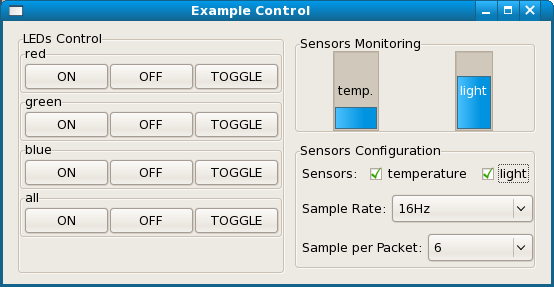
\includegraphics[scale=0.5]{figures/PC_appli.png}
\end{center}
\caption{Graphical User Interface}
\label{fig:pcappli}
\end{figure}

\end{document}
